%%%%%%%%%%%%%%%%%%%%%%%%%%%%%%%%%%%%%%%%%
% a0poster Portrait Poster
% LaTeX Template
% Version 1.0 (22/06/13)
%
% The a0poster class was created by:
% Gerlinde Kettl and Matthias Weiser (tex@kettl.de)
% 
% This template has been downloaded from:
% http://www.LaTeXTemplates.com
%
% License:
% CC BY-NC-SA 3.0 (http://creativecommons.org/licenses/by-nc-sa/3.0/)
%
%%%%%%%%%%%%%%%%%%%%%%%%%%%%%%%%%%%%%%%%%

%----------------------------------------------------------------------------------------
%	PACKAGES AND OTHER DOCUMENT CONFIGURATIONS
%----------------------------------------------------------------------------------------

\documentclass[a0,portrait]{a0poster}

\usepackage{multicol} % This is so we can have multiple columns of text side-by-side
\columnsep=100pt % This is the amount of white space between the columns in the poster
%\columnseprule=3pt % This is the thickness of the black line between the columns in the poster

\usepackage[svgnames,dvipsnames]{xcolor} % Specify colors by their 'svgnames', for a full list of all colors available see here: http://www.latextemplates.com/svgnames-colors

\usepackage{times} % Use the times font
%\usepackage{palatino} % Uncomment to use the Palatino font

\usepackage{graphicx} % Required for including images
\graphicspath{{figs/}} % Location of the graphics files
\usepackage{booktabs} % Top and bottom rules for table
\usepackage[font=small,labelfont=bf]{caption} % Required for specifying captions to tables and figures
\usepackage{amsfonts, amsmath, amsthm, amssymb} % For math fonts, symbols and environments
\usepackage{wrapfig} % Allows wrapping text around tables and figures
\usepackage{subcaption}
\usepackage{bm}
\usepackage{array}
\usepackage{amsmath,amssymb}
\usepackage{inconsolata}
\usepackage[T1]{fontenc}
\usepackage[scaled]{beramono}
\newcommand\Small{\fontsize{17}{19}\selectfont}
\newcommand*\LSTfont{\Small\ttfamily}
\usepackage{listings}
  \definecolor{mygreen}{rgb}{0,0.4,0}
  \lstset{
    language=Lisp,
    keywordstyle=\color{black},
    commentstyle=\color{mygreen},
    keywordstyle=[2]\color{RawSienna},
    keywords=[2]{ASSUME,PREDICT,INFER,OBSERVE,DEFINE},
    keywordstyle=[3]\color{black},
    keywords=[3]{tag,gamma,uniform-continuous,log,make-squaredexp,make-whitenoise,gpmem,mapv,first,repeat,do,mh,one,add-funcs,make-se,lambda,emulator,lookup,argma-of-array,linspace,run,array,pass,mc-argmax,uniform-structure,subset,lte,if,flip,mult-funcs,for,to},
    basicstyle=\LSTfont,
    literate=%
    {0}{{{\color{DarkBlue}0}}}1
    {1}{{{\color{DarkBlue}1}}}1
    {2}{{{\color{DarkBlue}2}}}1
    {3}{{{\color{DarkBlue}3}}}1
    {4}{{{\color{DarkBlue}4}}}1
    {5}{{{\color{DarkBlue}5}}}1
    {6}{{{\color{DarkBlue}6}}}1
    {7}{{{\color{DarkBlue}7}}}1
    {8}{{{\color{DarkBlue}8}}}1
    {9}{{{\color{DarkBlue}9}}}1
  }



\newcommand{\gpmem}{\texttt{gpmem}}
\newcommand{\compute}{{\textrm{compute}}}
\newcommand{\emu}{{\textrm{emu}}}
\newcommand{\restr}{{\textrm{restr}}}
\newcommand{\true}{{\textrm{true}}}
\newcommand{\rmnew}{{\textrm{new}}}
\newcommand{\past}{{\textrm{past}}}
\newcommand{\prior}{{\textrm{prior}}}
\newcommand{\noisy}{{\textrm{noisy}}}
\newcommand{\noise}{{\textrm{noise}}}

\newcommand{\Acal}{\mathcal{A}}
\newcommand{\R}{\mathbb{R}}

\newcommand{\abf}{\mathbf{a}}
\newcommand{\fbf}{\mathbf{f}}
\newcommand{\rbf}{\mathbf{r}}
\newcommand{\wbf}{\mathbf{w}}
\newcommand{\xbf}{\mathbf{x}}
\newcommand{\ybf}{\mathbf{y}}
\newcommand{\Kbf}{\mathbf{K}}
\newcommand{\Ibf}{\mathbf{I}}

\newcommand{\pn}[1]{\left( #1 \right)}
\newcommand{\bkt}[1]{\left[ #1 \right]}
\newcommand{\br}[1]{\left\{ #1 \right\}}
\newcommand{\abs}[1]{\left\lvert #1 \right\rvert}
\newcommand{\Ebkt}[2][]{\mathbb{E}_{#1}\bkt{#2}}
\newcommand{\mvert}{\ \middle\vert\ }

\DeclareMathOperator*{\Cov}{Cov}
\begin{document}

%----------------------------------------------------------------------------------------
%	POSTER HEADER 
%----------------------------------------------------------------------------------------

% The header is divided into two boxes:
% The first is 75% wide and houses the title, subtitle, names, university/organization and contact information
% The second is 25% wide and houses a logo for your university/organization or a photo of you
% The widths of these boxes can be easily edited to accommodate your content as you see fit
\begin{flushright}
\begin{minipage}[b]{0.25\linewidth}
\includegraphics[width=7cm]{mitlogo.png}
\hspace{1cm}
\includegraphics[width=8cm]{royalhollowaylogo.jpg}
\end{minipage} 
\end{flushright}

\vspace{2cm}

\begin{center}
\addtolength{\tabcolsep}{20pt} 
\veryHuge \textbf{Probabilistic Programming with Gaussian Process Memoization} \color{Black}\\[1.5cm] % Title
 \Large   \begin{tabular}{  c  c  c c}
           \textbf{Ulrich Schaechtle}  & \textbf{Ben Zinberg} & \textbf{Vikash K. Mansinghka} & \textbf{Kostas Stathis}\\ 
           Department of Computer Science & Computer Science \& AI Lab & Computer Science \& AI Lab & Department of Computer Science \\
           Royal Holloway, Univ. of London & Massachusetts Institute of Technology & Massachusetts Institute of Technology & Royal Holloway, Univ. of London \\
        \end{tabular}

\addtolength{\tabcolsep}{-2pt} 
\end{center}



\vspace{3cm} % A bit of extra whitespace between the header and poster content

%----------------------------------------------------------------------------------------

\begin{multicols}{3} % This is how many columns your poster will be broken into, a portrait poster is generally split into 2 columns

%----------------------------------------------------------------------------------------
%	ABSTRACT
%----------------------------------------------------------------------------------------

%\color{Navy} % Navy color for the abstract

\begin{abstract}
This paper describes the {\em Gaussian process memoizer}, a probabilistic programming technique that uses Gaussian processes to provides a statistical alternative to memorization. Memoizing a target procedure results in a ``self-caching'' wrapper that remembers previously computed values. Gaussian process memoization additionally produces a statistical emulator based on a Gaussian process whose predictions automatically improve whenever a new value of the target procedure becomes available. This paper also introduces  an efficient implementation, named {\tt gpmem}, that can use kernels given by a broad class of probabilistic programs. The flexibility of {\tt gpmem} is illustrated via three applications: (i) GP regression with hierarchical hyper-parameter learning, (ii) Bayesian structure learning via compositional kernels generated by a probabilistic grammar, and (iii) a bandit formulation of Bayesian optimization with automatic inference and action selection. All applications share a single 85-line Python library and require fewer than 20 lines of probabilistic code each.
\end{abstract}


\color{DarkSlateGray} % DarkSlateGray color for the rest of the content
%\color{SaddleBrown} % SaddleBrown color for the introduction
%----------------------------------------------------------------------------------------
%	GP Memoization
%----------------------------------------------------------------------------------------
\section*{GP Memoization: \texttt{gpmem}}
\subsection*{Gaussian Processes}
$f(\xbf)$ is the multivariate Gaussian $f(\xbf) \sim \mathcal{N}(0, k(\xbf,\xbf))$,
where $k(\xbf,\xbf') = \Cov_f\pn{f(\xbf), f(\xbf')}$ is the covariance function, a.k.a.\ kernel.
The marginal likelihood can be expressed as:
\begin{equation*}
\label{eq:marg}
p\pn{f(\xbf) = \ybf \mvert \xbf} = \int p\pn{f(\xbf) = \ybf \mvert f, \xbf}\, p(f|\xbf) \, df
\end{equation*}


\subsection*{A Variation on Memoization}
{\em GP memoization} produces two components:
\[ f \to (f_\compute, f_\emu) \]
\begin{itemize}
\setlength{\itemindent}{1cm}
 \item is a generalization of traditional memoization;
 \item changes semantics of a probabilistic program;
 \item $f_\emu$ is a statistical emulator with GP prior;
 \item each time $f_\compute$ is called, an observation is incorporated into $f_\emu$ and predictions improve.
\end{itemize}


---------------------------------------------------------------------


%----------------------------------------------------------------------------------------
%	Bayesian GP
%----------------------------------------------------------------------------------------
\section*{Bayesian GP}

We show how we can use  {\tt gpmem} to reproduce Neal's Hierarchical Bayesian GP regression~\cite{neal1997monte} for data with outliers.

\begin{center}
Regression on data set $D$ \\
$\Updownarrow$ \\
Statistical emulation of $f_\restr(x) = \begin{cases}
      D[x], & \text{if $x$ is a data point} \\
      \text{Error}, & \text{otherwise}
    \end{cases}$
\end{center}
\begin{minipage}{\linewidth}
\belowcaptionskip=-10pt
\begin{lstlisting}[frame=single,caption=Hierarchical  GP Smoothing,mathescape,label=alg:gphierarch]
;;; SETTING UP THE MODEL
ASSUME alpha-sf (tag 'hyperhyper (gamma 7 1))
ASSUME {{... several more hyper-hyperparameters ...}}
;; Parameters of the covariance function
ASSUME sf (tag 'hyper (log (gamma alpha-sf beta-sf)))
ASSUME l (tag 'hyper (log (gamma alpha-l beta-l)))
ASSUME sigma (tag 'hyper (uniform-continuous 0 2))
;; The covariance function
ASSUME se (make-squaredexp sf l)
ASSUME wn (make-whitenoise sigma)
ASSUME composite-covariance (add-funcs se wn)

;;; PERFORMING INFERENCE
;; Create a prober and emulator using gpmem
ASSUME f-restr (get-neal-prober)
ASSUME compute-and-emu (gpmem f-restr composite-covariance)

;; Probe all data points
PREDICT (mapv (first compute-and-emu) (get-neal-data-xs))

;; Infer hypers and hyperhypers
INFER (repeat 100 (do
    (mh 'hyperhyper one 2)
    (mh 'hyper one 1)))

\end{lstlisting}
\end{minipage}
Observed data is generated with the following model: 
\begin{equation*}
f(x) =  0.3 + 0.4 x + 0.5 \sin(2.7x) + \frac{1.1}{(1+ x^2)} + \eta \;\;\; \text{with}\;\;\eta \sim \mathcal{N}(0,\sigma)
\end{equation*} where $\sigma = 0.1$ with probability $0.95$, $\sigma = 1$ otherwise.
\begin{center}
\includegraphics[width=6cm]{neal_se_1final.png}
\includegraphics[width=6cm]{neal_se_2final.png}
\includegraphics[width=6cm]{neal_se_3final.png}
\captionof{figure}{\color{DarkSlateGray} (left to right) predictions before data has been observed, after data has been observed, and after we inferred the hyperparameters}
\end{center}


% Left or right alignment is specified in the first bracket, the width of the table is in the second


%\begin{wraptable}{r}{15cm} 
\begin{center}
%\includegraphics[width=10cm]{neal_contour_l_vs_sf_s__marginal_before.png}
\includegraphics[width=7cm]{neal_contour_l_vs_sf_s__marginal_after.png} 
\captionof{figure}{\color{DarkSlateGray}  Contour plot and marginals of the the $\ell$ and $\theta$ hyper-parameters of the above program after inference}
\end{center}

\vfill
\columnbreak


%----------------------------------------------------------------------------------------
%	Learning of Symbolic Structure
%----------------------------------------------------------------------------------------
\section*{GP Structure Learning}

 \begin{center} 
\begin{tabular}{m{11.5cm} m{4cm}}
$SE = \sigma^2 \exp(-\frac{(x-x^\prime)^2}{2\ell^2})$&\includegraphics[width=4cm]{gpSamples/se.png}\\
$LIN = \theta (x x^\prime)$&\includegraphics[width=4cm]{gpSamples/lin.png}\\
$PER = \theta \exp \bigg( \frac{2 \sin^2 ( \pi (x - x^\prime)/p}{\ell^2} \bigg)$&\includegraphics[width=4cm]{gpSamples/per.png}\\
$RQ =   \theta \bigg(1 + \frac{(x - x^\prime)^2}{2 \alpha \ell^2} \bigg)^{-\alpha}$&\includegraphics[width=4cm]{gpSamples/rq.png}
\end{tabular}
\end{center}
\subsection*{Kernel Composition}
\begin{equation*}
\mathbf{K}_{\textrm{new}} = \mathbf{K}_1 + \mathbf{K}_2 \;\;\;\;\;\;\text{or}\;\;\;\;\;\; \mathbf{K}_{\textrm{new}} = \mathbf{K}_1 \times \mathbf{K}_2 
\end{equation*}
\begin{minipage}{\linewidth}
\small
\begin{lstlisting}[frame=single,label=alg:structureVent,caption=Venture Code for Bayesian GP Structure Learning,mathescape]
;;; GRAMMAR FOR KERNEL STRUCTURE
ASSUME base-kernels (list K$_1$,K$_2$,$\cdots$,K$_n$) ;; defined as above

;; prior on the number of kernels
ASSUME p-number-k (tag 'number-kernels (uniform-structure n))
ASSUME s (tag 'choice-subset (subset  base-kernels p-number-k)) 

ASSUME composition (tag 'composit (lambda (l) ;; kernel composition
                     (if (lte ( size l) 1)
                         (first l)
                          (if (flip)
                              (add-funcs (first l) (cov-compo (rest l)))
                              (mult-funcs (first l) (cov-compo (rest l)))
                          ))))
                          
ASSUME K (composition  s)

ASSUME (list f-compute f-emu) (gpmem f-restr K )

PREDICT (mapv f-compute (get-data-xs)) ;; probe all data points

;;; PERFORMING INFERENCE  
INFER  (repeat 2000 (do
                        (mh 'number-kernel one 1) 
                        (mh 'choice-subset one 1) 
                        (mh 'composit one 1) 
                        (mh 'hyper one 10)))
\end{lstlisting}

\end{minipage}



 
 \subsection*{Results}
 500 samples drawn from the posterior on structure for the CO2 dataset used in the Automated Statistician Project~\cite{duvenaud2013structure}:
 \begin{center}\vspace{1cm}
%\includegraphics[width=0.7\linewidth]{structureCo2b.png}
%\captionof{figure}{\color{DarkSlateGray} Composition of covariance function parsed using the example SE $\times$ LIN $+$ PER $\times$ LIN $+$  RQ $\times$ LIN}
\includegraphics[width=0.7\linewidth]{structureCo2b.png}
\end{center}\vspace{1cm}
Posterior samples for curves for the airline dataset where SE $\times$ LIN $+$ PER $\times$ LIN $+$  RQ $\times$ LIN is sampled from the structure grammar:
 \begin{center}\vspace{1cm}
\includegraphics[width=\linewidth]{rawx.png}\\
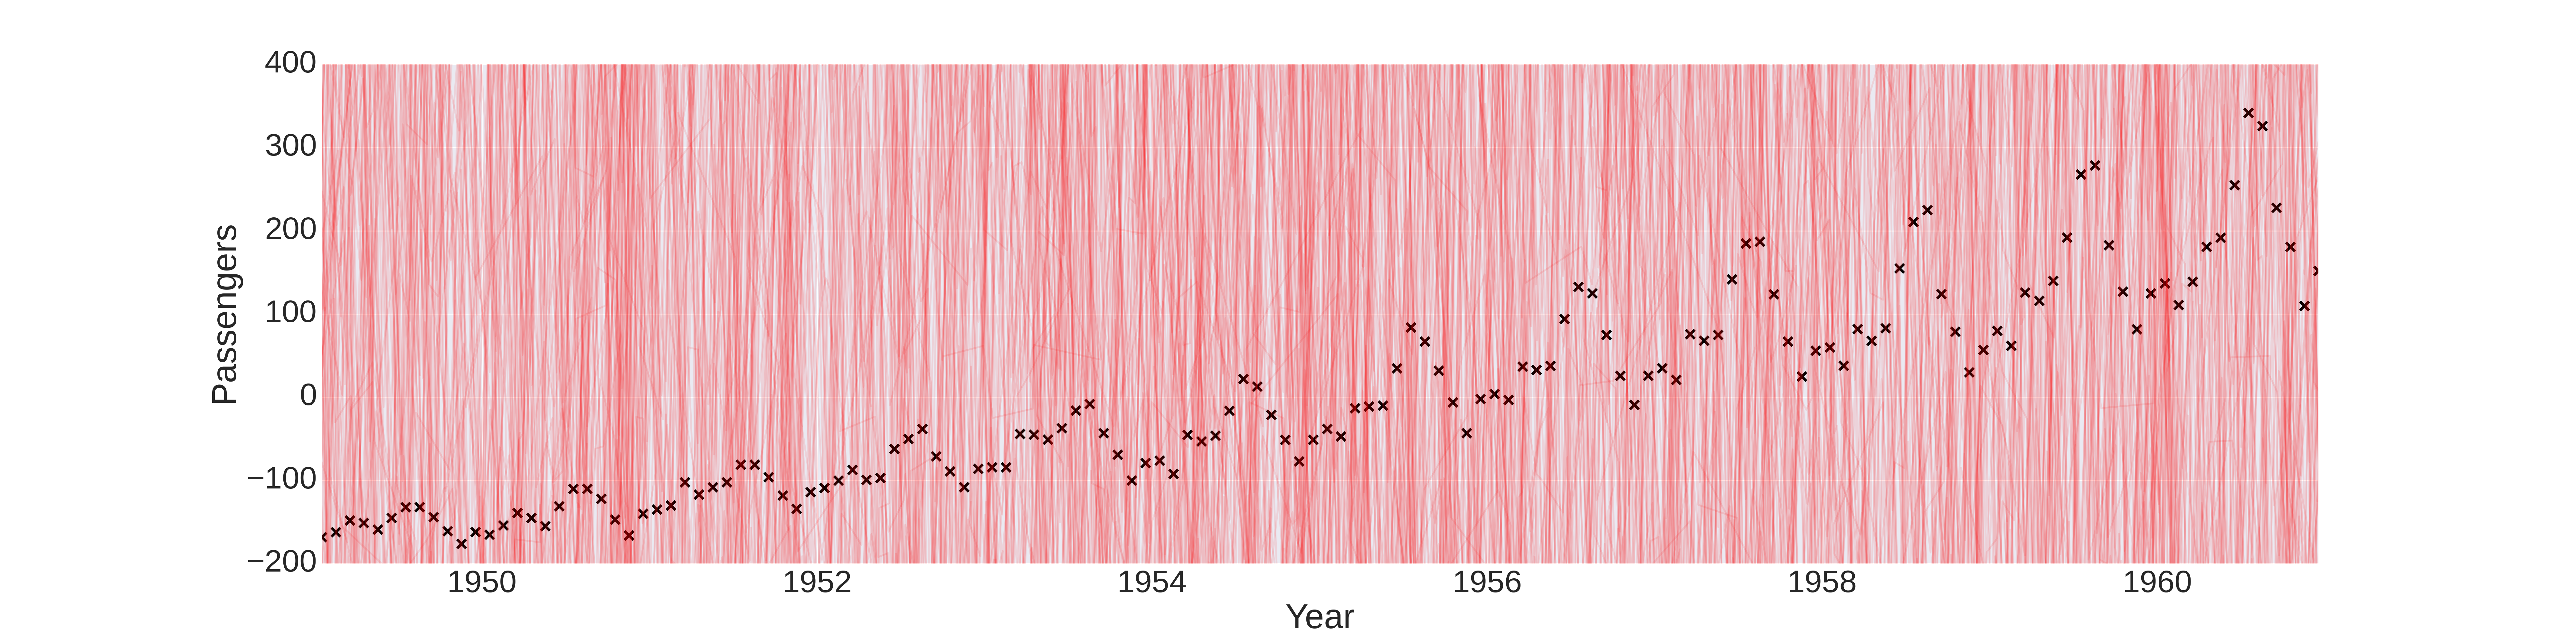
\includegraphics[width=\linewidth]{priorx.png}\\
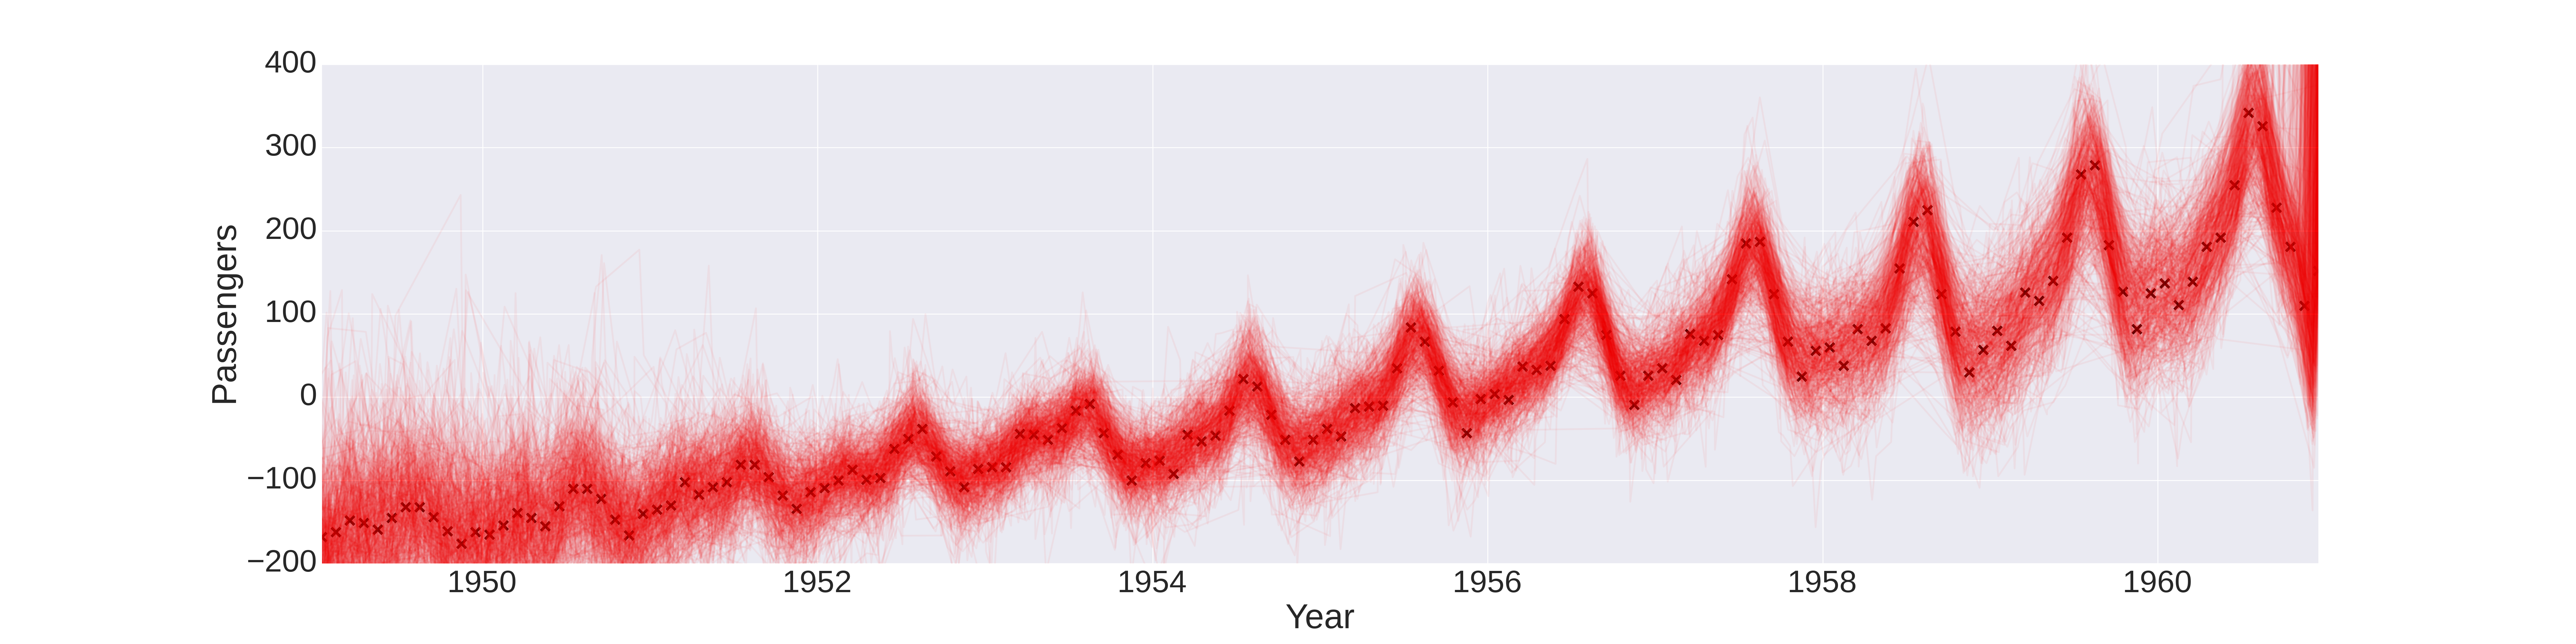
\includegraphics[width=\linewidth]{posteriorx.png}
\captionof{figure}{\color{DarkSlateGray} Top: raw data, monthly airline passengers. Middle, prior on functions. Bottom, posterior.}
\end{center}


\subsection*{Decomposing a candidate Structure}
\begin{center}\vspace{1cm}
\includegraphics[width=0.7\linewidth]{parseTree.pdf}
%\captionof{figure}{\color{DarkSlateGray} Composition of covariance function parsed using the example SE $\times$ LIN $+$ PER $\times$ LIN $+$  RQ $\times$ LIN}
\end{center}\vspace{1cm}
 
\vfill
\columnbreak
%----------------------------------------------------------------------------------------
%	Bayesian Optimization
%----------------------------------------------------------------------------------------
\section*{Bayesian Optimization}

\begin{minipage}{\linewidth}
\begin{lstlisting}[frame=single,label=alg:structureVent,caption=Venture Code for Bayesian Optimization,mathescape]
ASSUME sf1 (tag 'hyper (log (uniform-continuous 0 10)))
ASSUME l1 (tag 'hyper (log (uniform-continuous 0 10)))
ASSUME se (make-se sf1 l1)
ASSUME blackbox-f (get-bayesopt-blackbox)
ASSUME compute-and-emu (gpmem blackbox-f se)

DEFINE get-uniform-candidate 
	(lambda (prev-xs) (uniform-continuous -20 20))
DEFINE mc-argmax
        (lambda (emulator prev-xs)
             ((lambda (candidate-xs)
                (lookup candidate-xs
                        (argmax-of-array (mapv emulator candidate-xs))))
              (mapv (lambda (i) (get-uniform-candidate prev-xs))
                   (linspace 0 19 20))))
DEFINE emulator-point-sample
        (lambda (x)
          (run (sample
            (lookup ((second compute-and-emu) (array ,x))
                    0))))

INFER
    (repeat 15 (do pass

      ;; Call f-compute on the next probe point
      (PREDICT ((first compute-and-emu)
                ,(mc-argmax emulator-point-sample '-)))
                
      ;; Hyperparameter inference
      (mh 'hyper one 50)))
\end{lstlisting}
\end{minipage}
      
%Bayesian Optimization with Thompson sampling providing:
%\begin{itemize}
% \item  the ability to search over a broader space of contexts than the parametric families that are typically used;
% \item parsimony of the resulting probabilistic program.
%\end{itemize}
\subsection*{Thompson Sampling for Homogeneous Sequential Markov Decision Processes}



\includegraphics[width=20cm]{BayesOpt_gpmem_sequence.png}


\subsection*{Above: Dynamics of Thompson sampling}
\begin{itemize}
 \item the blue curve is the true function $V$;
 \item the red region is a blending of 100 samples of the curve generated (jointly) by a GP-based emulator $V_\emu$;
 \item  the left and right columns show the state of $V_\emu$ before and after hyperparameter inference
 \item in the right column, the next chosen probe point is circled in green;
 \item each successive probe point $a$ is the (stochastic) maximum of $V_\emu$, sampled pointwise and conditioned on the values of the previously probed points; and
 \item probes tend to happen at points either where the value of $V_\emu$ is high, or where $V_\emu$ has high uncertainty.
\end{itemize}

     
     
%
%\begin{center}\vspace{1cm}
%\captionof{figure}{\color{DarkSlateGray} } \label{fig:bayesopt-sequence}
%\end{center}

   



%\section*{Conclusions}
%{\tt gpmem} is a generalization of a number of GP\newline related models and can be applied to:
%\begin{itemize}
%\setlength{\itemindent}{1cm}
%\item Hierarchical Bayesian GP
%\item Kernel Structure Learning
%\item Bayesian Optimization
%\end{itemize}

\color{DarkSlateGray} % Set the color back to DarkSlateGray for the rest of the content

%----------------------------------------------------------------------------------------
%	FORTHCOMING RESEARCH
%----------------------------------------------------------------------------------------

%\section*{Forthcoming Research}

%Vivamus molestie, risus tempor vehicula mattis, libero arcu volutpat purus, sed blandit sem nibh eget turpis. Maecenas rutrum dui %blandit lorem vulputate gravida. Praesent venenatis mi vel lorem tempor at varius diam sagittis. Nam eu leo id turpis interdum %luctus a sed augue. Nam tellus.

 %----------------------------------------------------------------------------------------
%	REFERENCES
%----------------------------------------------------------------------------------------
\small

\bibliographystyle{plain} % Plain referencing style
\bibliography{June2015} % Use the example bibliography file sample.bib

%----------------------------------------------------------------------------------------
%	ACKNOWLEDGEMENTS
%----------------------------------------------------------------------------------------

%\section*{Acknowledgements}


%----------------------------------------------------------------------------------------

\end{multicols}
\end{document}
